\documentclass[12pt]{article}

\usepackage{amsmath,amsthm,amsfonts,amssymb,amsxtra}
\usepackage{tikz,array}
\usetikzlibrary{arrows}
\renewcommand{\theenumi}{(\alph{enumi})} 
\renewcommand{\labelenumi}{\theenumi}

\pagestyle{empty}
\setlength{\textwidth}{7in}
\setlength{\oddsidemargin}{-0.5in}
\setlength{\topmargin}{-1.0in}
\setlength{\textheight}{9.5in}

\theoremstyle{definition}
\newtheorem{problem}{Problem}

\begin{document}

\noindent{\large\bf MATH 242}\hfill{\large\bf Test \#3}\hfill{\large\bf
  Spring 2018}\hfill{\large\bf Page 1/6}\hrule

\bigskip
\begin{center}
  \begin{tabular}{|ll|}
    \hline & \cr
    {\bf Name: } & \makebox[12cm]{\hrulefill}\cr & \cr
    {\bf VIP ID:} & \makebox[12cm]{\hrulefill}\cr & \cr
    \hline
  \end{tabular}
\end{center}
\begin{itemize}
\item Write your name and your VIP ID in the space provided above.
\item The test has six (6) pages, including this one and a formula sheet at the end.
\item \textbf{Do not detach} the formula sheet from the booklet.
\item Show sufficient work to justify all answers unless otherwise stated in the problem.  Correct answers with inconsistent work may not be given credit.
\item Credit for each problem is given at the right of each problem number.
\end{itemize}
\hrule

\begin{center}
  \begin{tabular}{|c|c|c|}
    \hline
    &&\cr
    {\large\bf Page} & {\large\bf Max} & {\large\bf Points} \cr
    &&\cr
    \hline
    &&\cr
    {\Large 2} & \Large 20 & \cr
    &&\cr
    \hline
    &&\cr
    {\Large 3} & \Large 30 & \cr
    &&\cr
    \hline
    &&\cr
    {\Large 4} & \Large 30 & \cr
    &&\cr
    \hline
    &&\cr
    {\Large 5} & \Large 20 & \cr
    &&\cr
    \hline\hline
    &&\cr
    {\large\bf Total} & \Large 100 & \cr
    &&\cr
    \hline
  \end{tabular}
\end{center}
\newpage

%%%%%%%%%%%%%%%%%%%%%%%%%%%%%%%%%%%%% Page 2
\noindent{\large\bf MATH 242}\hfill{\large\bf Test \#3}\hfill{\large\bf Spring 2018}\hfill{\large\bf Page 2/6}\hrule

\bigskip
\begin{problem}[10 pts]
Suppose that the population of a country satisfies a logistic equation.  The limiting population is 200 million people.  In 1940, there were 100 million people, and were then growing at a rate of one million people a year.   Predict the population in the year 2020.
\vspace{6cm}
\begin{flushright}
\begin{tikzpicture}
\draw (-2cm, 0.5cm) node{Population in 2020:};
\draw (0cm,-0.2cm) rectangle (5cm,1.2cm);
\end{tikzpicture}
\end{flushright}
\end{problem} 
\hrule

\begin{problem}[10 pts]
Plot a slope field to indicate the stability of the following population model:
\begin{equation*}
\frac{dP}{dt} = (P-1)^3(P-3)^2(2P^2-13P+15)
\end{equation*}
\end{problem}

\newpage

%%%%%%%%%%%%%%%%%%%%%%%%%%%%%%%%%%%%% Page 3
\noindent{\large\bf MATH 242}\hfill{\large\bf Test \#3}\hfill{\large\bf
  Spring 2018}\hfill{\large\bf Page 3/6}\hrule

\bigskip
\begin{problem}[10 pts each]
Suppose that at time $t=0$, half of a logistic population of 100,000 persons have heard a certain rumor, and that the number of those who have heard it is then increasing­ at the rate of 1000 persons per day. How long will it take for this rumor to spread to 80\% of the population?
\vspace{4cm}
\begin{flushright}
\begin{tikzpicture}
\draw (0cm,-0.2cm) rectangle (3cm,1.2cm);
\end{tikzpicture}
\end{flushright}
\end{problem}
\hrule

\begin{problem}[20 pts---10 pts each part]
Suppose that the number $P(t)$ of alligators in a swamp after $t$ months satisfies the differential equation 
\begin{equation*}
\frac{dP}{dt} = 0.0001 P^2 - 0.01 P.
\end{equation*}
\begin{enumerate}
  \item If initially there were 25 alligators in the swamp, solve this differential equation to determine what happens to the alligator population in the long run.
\vspace{3.5cm}
\begin{flushright}
\begin{tikzpicture}
\draw (0cm,-0.2cm) rectangle (3cm,1.2cm);
\end{tikzpicture}
\end{flushright}
  \item Repeat the previous part, except with 150 alligators initially.
\vspace{3.5cm}
\begin{flushright}
\begin{tikzpicture}
\draw (0cm,-0.2cm) rectangle (3cm,1.2cm);
\end{tikzpicture}
\end{flushright}
\end{enumerate}
\end{problem}

\newpage

%%%%%%%%%%%%%%%%%%%%%%%%%%%%%%%%%%%%% Page 4
\noindent{\large\bf MATH 242}\hfill{\large\bf Test \#3}\hfill{\large\bf
  Spring 2018}\hfill{\large\bf Page 4/6}\hrule

\bigskip
\begin{problem}[10 pts]
Find the family of curves for which the length of the part of the tangent between the point of contact $(x,y)$ and the $y$--axis is equal to the $y$--intercept of the tangent.
\vspace{4cm}
\begin{flushright}
\begin{tikzpicture}
\draw (0cm,-0.2cm) rectangle (5cm,1.2cm);
\end{tikzpicture}
\end{flushright}
\end{problem}
\hrule

\begin{problem}[20 pts---10 pts each]
Find the orthogonal trajectories of each of the following families of curves:
\begin{enumerate}
  \item $3x+5y = k$
  \vspace{3.5cm}
  \begin{flushright}
  \begin{tikzpicture}
  \draw (0cm,-0.2cm) rectangle (5cm,1.2cm);
  \end{tikzpicture}
  \end{flushright}
  \item $y = 3x- 4 + ke^{-5x}$
  \vspace{3.5cm}
  \begin{flushright}
  \begin{tikzpicture}
  \draw (0cm,-0.2cm) rectangle (5cm,1.2cm);
  \end{tikzpicture}
  \end{flushright}
\end{enumerate}
\end{problem}

\newpage

%%%%%%%%%%%%%%%%%%%%%%%%%%%%%%%%%%%%% Page 5
\noindent{\large\bf MATH 242}\hfill{\large\bf Test \#3}\hfill{\large\bf
  Spring 2018}\hfill{\large\bf Page 5/6}\hrule

\bigskip
\begin{problem}[10 pts]
Find all curves for which the subtangent at any point $(x,y)$ is equal to five times the square of the abscissa.
\vspace{8cm}
\begin{flushright}
  \begin{tikzpicture}
  \draw (0cm,-0.2cm) rectangle (5cm,1.2cm);
  \end{tikzpicture}
  \end{flushright}
\end{problem}
\hrule
\begin{problem}[10 pts]
Find all curves for which the part of the normal drawn at point $(x,y)$ between this point and the $x$--axis is bisected by the $y$--axis.
\vspace{8cm}
\begin{flushright}
  \begin{tikzpicture}
  \draw (0cm,-0.2cm) rectangle (5cm,1.2cm);
  \end{tikzpicture}
  \end{flushright}
\end{problem}

\newpage

%%%%%%%%%%%%%%%%%%%%%%%%%%%%%%%%%%%%% Page 6
\noindent{\large\bf MATH 242}\hfill{\large\bf Test \#3}\hfill{\large\bf
  Spring 2018}\hfill{\large\bf Page 6/6}\hrule

\bigskip
{\Large Formula Sheet}

\begin{center}
%\includegraphics[width=\linewidth]{table.pdf}
\begin{tikzpicture}
  \node[scale=0.97]{
 \begin{tabular}{|m{1.2cm}|m{4.3cm}l||m{2.1cm}|m{4.3cm}l|}
 \hline
    $f(x)$\raisebox{0.5cm} & $\mathcal{L}\{f\}=\int_0^\infty e^{-sx}f(x)\, dx$\raisebox{0.5cm} & &
    \raisebox{0.5cm} & \raisebox{0.5cm} & \\[0.4cm] 
    \hline \hline
    $1$ & $\dfrac{1}{s}$\raisebox{0.6cm} & $s>0$ &
    $cf(x)\pm g(x)$ & $cF(s) \pm G(s)$\raisebox{0.4cm} & $s>max(a,b)$ \\[0.4cm]
    \hline
    $x^n$ & $\dfrac{n!}{s^{n+1}}$\raisebox{0.6cm} & $s>0$ & $e^{\alpha x}f(x)$ & $F(s-\alpha)$\raisebox{0.4cm} & $s>a+\alpha$ \\[0.4cm]
    \hline
    $e^{\alpha x}$ & $\dfrac{1}{s-\alpha}$\raisebox{0.6cm} & $s>\alpha$ &
    $x^n f(x)$ & $(-1)^n F^{(n)}(s)$\raisebox{0.4cm} & $s>a$ \\[0.4cm]
    \hline
    $\sin \beta x$ & $\dfrac{\beta}{s^2+\beta^2}$\raisebox{0.6cm} & $s>0$ & $f'(x)$ & $s F(s) -f(0)$\raisebox{0.4cm} & \\[0.4cm]
    \hline
    $\cos \beta x$ & $\dfrac{s}{s^2+\beta^2}$\raisebox{0.6cm} & $s>0$ &$f''(x)$\raisebox{0.4cm} & $s^2F(s) - sf(0)  - f'(0)$ & \\[0.4cm]
    \hline
    \end{tabular} };
    \end{tikzpicture}
\end{center}

\begin{itemize}
\item The slope of the tangent line to the curve at $(x_0,y_0)$ is $f'(x_0)$.
\item The slope of the normal line to the cure at $(x_0,y_0)$ is $-1/f'(x_0)$.
\item The equation of the tangent line at $(x_0,y_0)$ is $y-y_0=y'(x-x_0)$.
\item The equation of the normal line at $(x_0,y_0)$ is $y-y_0 = (x_0-x)/f'(x_0)$.
\item The $x$--intercept of the tangent is $x_0-f(x_0)/f'(x_0)$.
\item The $y$--intercept of the tangent is $f(x_0)-x_0 f'(x_0)$.
\item The $x$--intercept of the normal is $x_0+f(x_0)f'(x_0)$.
\item The $y$--intercept of the normal is $f(x_0)+x_0/f'(x_0)$.
\item The length of the tangent between $(x_0,y_0)$ and the $x$--axis is $\lvert y_0 \rvert\sqrt{1+1/f'(x_0)^2}$.
\item The length of the tangent between $(x_0,y_0)$ and the $y$--axis is $\lvert x_0 \rvert\sqrt{1+f'(x_0)^2}$.
\item The length of the normal between $(x_0,y_0)$ and the $x$--axis is $\lvert y_0 \rvert\sqrt{1+f'(x_0)^2}$.
\item The length of the normal between $(x_0,y_0)$ and the $y$--axis is $\lvert x_0 \rvert \sqrt{1+1/f'(x_0)^2}$.
\item The length of the subtangent is $\lvert f(x_0)/f'(x_0) \rvert$.
\item The length of the subnormal is $\lvert f(x_0) f'(x_0) \rvert$.
\end{itemize}



\end{document}
